%!TEX root = ../../../root.tex

\begin{figure}[H]
	\centering
	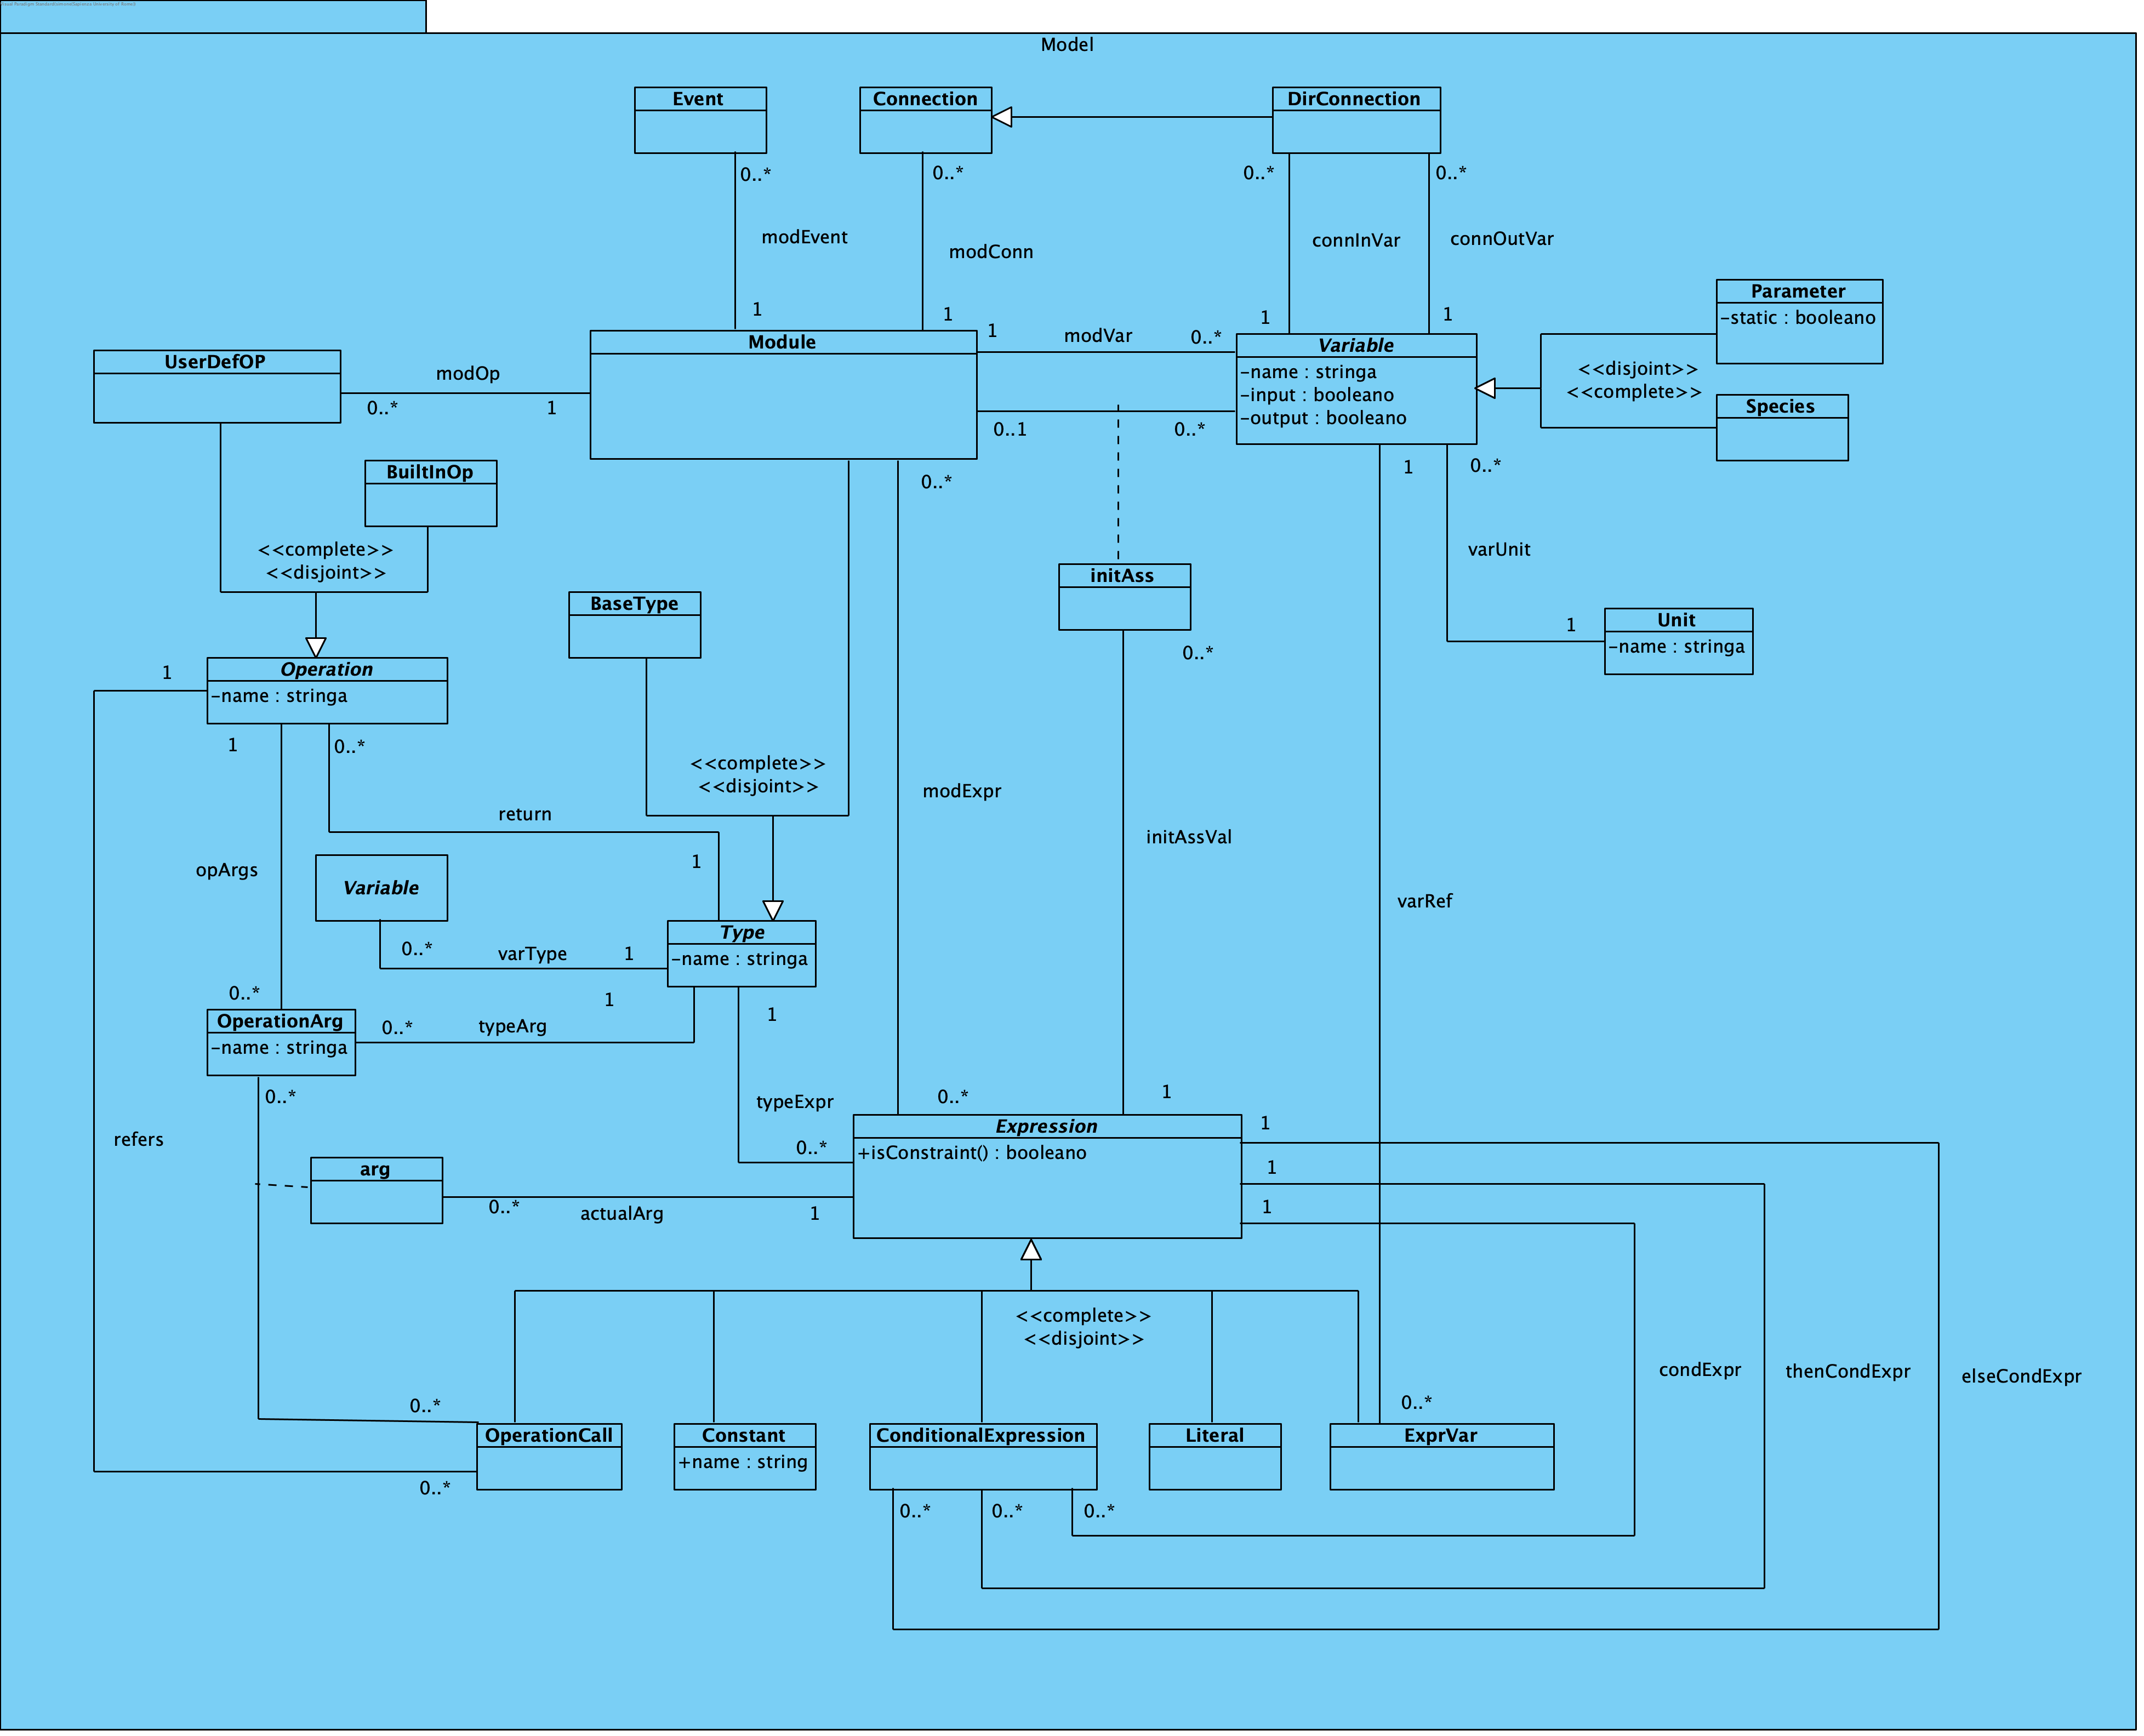
\includegraphics[width=\textwidth]{ModelAnalysis.png}
	\caption{\small{\textit{Conceptual Analysis: Package Model.}}}
\end{figure}

\InputSection[sec:modelstranslator:analysis:model_analysis:module]{Classe Module}{Module/content.tex}
\InputSection[sec:modelstranslator:analysis:model_analysis:variable]{Classe Variable}{Variable/content.tex}
\InputSection[sec:modelstranslator:analysis:model_analysis:type]{Classe Type}{Type/content.tex}
\InputSection[sec:modelstranslator:analysis:model_analysis:unit]{Classe Unit}{Unit/content.tex}
\InputSection[sec:modelstranslator:analysis:model_analysis:operation]{Classe Operation}{Operation/content.tex}
\InputSection[sec:modelstranslator:analysis:model_analysis:connection]{Classe Connection}{Connection/content.tex}
\InputSection[sec:modelstranslator:analysis:model_analysis:event]{Classe Event}{Event/content.tex}
\InputSection[sec:modelstranslator:analysis:model_analysis:expression]{Classe Expression}{Expression/content.tex}
